\chapter{Technischer Stand des Robotersystems}
In diesem Kapitel wird der, in Abschnitt~\ref{sec:motivation} referenzierter kollaborierender Schweißrobotersystem des Fraunhofer Institutes für Produktions- und Automatisierungstechnik en détail untersucht und seine Funktionsweise erklärt. Hierbei liegt der Fokus nicht nur auf dem Roboter, sondern auch auf die anderen mitwirkenden Hardware- sowie Softwarekomponenten des Systems.

\section{Die Roboterzelle}

\begin{figure}[b!]
	\includegraphics[width = \textwidth]{Abbildungen/roboter_zelle.png}
	\centering
	\caption{Die Roboterzelle}
\end{figure}
\emph{Zelle} wird hier als ein Oberbegriff für die restlichen Komponenten des Schweißrobotersystems verwendet. Der Grund für die Verwendung dieses Begriffs liegt daran, dass der Roboter sich in einem geschlossenem Raum mit den anderen Komponenten befindet und zusammen mit den als eine Einheit agiert. Der Cobot ist auf einem Metalltisch festmontiert, der auch als den Arbeitsplatz des Roboters sowie die elektrische Masse für das Schweißverfahren dient. Zu schweißende metallische Werkstücke werden auf dem Tisch fixiert und haben aufgrund des direkten Kontaktes mit der elektrische Masse ein Potential von null. Außer dem Schweißtisch befinden sich in der Zelle auch anderen Komponenten, die zum Schweißen erforderlich sind, sensorischen Zwecke erfüllen oder zur Gewährleistung der Sicherheit dienen. Die Schweißquelle, Drahtvorschubeinrichtung und Schutzgaszylinder befinden sich in diese Zelle und sind mittels Kabel und Schläuche mit der Schweißpistole verbunden. Die Kabel für Stromführung und Schläuche für die Überführung des Schutzgases und Schweißzusatzes werden zusammen gebündelt und zu der Schweißpistole so geführt, dass sie möglichst entfernt von den Roboterarmen sind. Dieses Bündel wird mittels gefederten Seilrollen, die an der Decke montiert und horizontal fahrbar sind, weit über den Roboter gehalten. Somit kann der Roboter während eines Bewegungsvorganges in beliebigen Richtungen ohne Hindernisse fahren. Am Endeffektor des Roboters ist auch ein Lasersensor fixiert, welches für die optische Sinnesempfindung verwendet wird. Der Sensor wird über den M8 8-Pin Anschluss an dem Roboterarm mit der Steuerung und über einen Ethernet-Kabel mit einem leistungsstarken Rechner, ein Industrie-PC (IPC), verbindet. Dieses Kabel wird auch mit den restlichen Kabeln zusammen gebündelt und von den Roboterarmen ferngehalten. Schließlich die Sicherheitsvorrichtungen, die bezugnehmend auf Abschnitt~\ref{ssec:cobots} dem Mitarbeiter schützen sollen. Die Einzelkomponenten der Roboterzelle werden jeweils detaillierter betrachtet

\subsection{Der Roboter}
Der Roboter dieses Systems ist die zentrale Hardwarekomponente dieses Systems. Dieser ist für die Bewegung und Handhabung der Schweißpistole und des Lasersensors zuständig. Verwendet wird hierfür ein sechs achsiges kollaborierender Roboter mit der Bezeichnung 10e von dem dänischen Unternehmen \emph{Universal Robots}. Mit einer Reichweite von 1300 mm und eine Traglast von 12,5 kg eignet sich der Cobot für die Bearbeitung größerer Werkstücke. Um die notwendigen Sicherheitsanforderung zu gewährleisten, kann dieser Cobot mit verschiedenen Sicherheitsfunktionen konfiguriert werden. Auch zur Kraftmessung und Kollisionserkennung ist er mit Kraft-Moment-Sensoren ausgestattet. Diese können Kräfte bis zu 100 N oder Momente bis zu 10 Nm mit einer Genauigkeit von 5,5 N beziehungsweise 0,5 Nm und einer diskreten Auflösung von 5,0N beziehungsweise 0,2 Nm in allen dreidimensionalen Richtungen ermessen. Jeder der sechs Achsen hat einen Arbeitsradius von $\pm \ang{360}$, allerdings sind die jeweiligen maximalen Geschwindigkeiten abweichend. Der Fußgelenk und der Schultergelenk können maximal $\pm \ang{120} s^{-1}$ in beiden Laufrichtungen drehen. Im Gegensatz dazu haben die drei Handgelenke eine maximale Rotationsgeschwindigkeit von $\pm \ang{180} s^{-1}$. Der Roboter hat eine Wiederholgenauigkeit von $\pm 0,05 mm$. Laut dem Hersteller ist es möglich, jeden möglichen Endeffektor mit dem richtigen Aufsatz am Roboterende zu montieren .Mit einem standardisierten M8 8-Pin Anschluss dürfen diese Endeffektoren oder andere Sensoren mit dem Roboter interagieren. Über den 8-Pin Stecker wird werden diese Geräte auch mit einem Strom beliefert. Eine Interaktion mit dem Werkzeug kann über die vorhandenen digitalen oder analogen Ein- und Ausgänge erfolgen. 

Die Steuereinheit des Roboters befindet sich in einem Schaltkasten, der mit dem Roboter über einen Kabel verbunden wird. Dieser Kabel liefert nicht nur den Strom zum Roboter, sondern ermöglicht es der Steuereinheit, Steuersignale zu senden und digitale sowie analoge Signale zu empfangen. Der Schaltkasten mit der Steuereinheit verfügt auch über jeweils sechzehn digitale Eingänge und Ausgänge sowie zwei analoge. Diese dienen als Schnittstelle zur Kommunikation mit anderen Geräte wie Lichtschranke, Notaustaster oder andere speicherprogrammierbare Steuerungen. Es verfügt auch über eine Ethernet-Schnittstelle zur Kommunikation mit anderen Rechnern über TCP/IP sowie zwecks der Fernsteuerung. Der Schaltkasten wird über einen Ethernet-Kabel mit dem IPC vernetzt.

Als letztes ist auch kleiner Tablett, das Teach-In-Pendant mit dem Schaltkasten verbunden. Auf diesem Pendant läuft die vorinstallierte Software zur Programmierung des Roboters, und bietet über einen Touch-Bildschirm die Möglichkeit der Interaktion an. Daneben befindet sich auch eine Notaustaste auf dem Tablett zum sofortigen Aufhalten des Roboters. Ein anderer Knopf, der sich auch am Roboter befindet, lässt beim Eindrücken eine einfache Positionierung und Bewegung des Roboters per Handführen. 

Die technischen Daten des Roboters wurden aus dem Produktdatenblatt sowie die Bedienungsanleitung erhoben.

%\subsection{Die Zelle}
%\emph{Zelle} wird hier als ein Oberbegriff für die restlichen Komponenten des Schweißrobotersystems verwendet. Der Grund für die Verwendung dieses Begriffs liegt daran, dass der Roboter sich in einem geschlossenem Raum mit den anderen Komponenten befindet und zusammen mit den als eine Einheit agiert. Der Cobot ist auf einem Metalltisch festmontiert, der auch als den Arbeitsplatz des Roboters sowie die elektrische Masse für das Schweißverfahren dient. Zu schweißende metallische Werkstücke werden auf dem Tisch fixiert und haben aufgrund des direkten Kontaktes mit der elektrische Masse ein Potential von null. Außer dem Schweißtisch befinden sich in der Zelle auch anderen Komponenten, die zum Schweißen erforderlich sind, sensorischen Zwecke erfüllen oder zur Gewährleistung der Sicherheit da stehen. Die Schweißquelle, Drahtvorschubeinrichtung und Schutzgaszylinder befinden sich in diese Zelle und sind mittels Kabel und Schläuche mit der Schweißpistole verbunden. Die Kabel für Stromführung und Schläuche für die Überführung des Schutzgases und Schweißzusatzes werden zusammen gebündelt und zu der Schweißpistole so geführt, dass sie möglichst entfernt von den Roboterarmen sind. Dieses Bündel wird mittels gefederten Seilrollen, die an der Decke montiert und horizontal fahrbar sind, weit über den Roboter gehalten. Somit kann der Roboter während eines Bewegungsvorganges in beliebigen Richtungen ohne Hindernisse fahren. Am Endeffektor des Roboters ist auch ein Lasersensor fixiert, welches für die optische Sinnesempfindung verwendet wird. Der Sensor wird über den M8 8-Pin Anschluss an dem Roboterarm mit der Steuerung und über einen Ethernet-Kabel mit einem Rechner verbindet. Dieses Kabel wird auch mit den restlichen Kabeln zusammen gebündelt und von den Roboterarmen ferngehalten. Eine detaillierte Behandlung des Sensors ist in Abschnitt~\ref{sec:lasersensor} zu finden. Schließlich die Sicherheitsvorrichtungen, die bezugnehmend auf Abschnitt~\ref{ssec:cobots} dem Mitarbeiter schützen sollen. 

\subsection{Sicherheitsvorrichtungen}
Zuerst sind die Sicherheitsfunktionen des Roboters zu betrachten. Es lässt sich die Bewegungsmöglichkeiten, maximale Gelenk- sowie Robotergeschwindigkeiten des Ellbogens, Endeffektors und der Mitte, und  maximales Drehmoment des Roboters auf benutzerdefinierte Werte einschränken. Weiterhin lässt sich der Roboter in Notfällen in verschiedenen Weisen aufhalten, beispielsweise mit einem Notschalter oder einer Abschaltung durch das System. Der Roboter kann auch in einem \emph{reduzierten} Modus betrieben werden. Es sollen Grenzwerte für die Geschwindigkeit, Kräfte und Momente des Roboters vordefiniert werden, die beim Aktivieren des Modus innerhalb von 500 ms übernommen werden. Dieser Modus kann entweder automatisch durch die Vordefinition einer Auslöseebene innerhalb des Roboter-Koordinatensystems oder durch einem anderen Gerät aktiviert werden. Wenn der Roboter die Grenze der Auslöseebene überschreitet, wird dieser Modus automatisch eingeschaltet. 

Zum Schutz vor dem gesundheitsschädlichen Schweißrauch, wird ein Filter- und Absauggerät der Firma Kemper GmbH. Dieses Gerät entfernt die beim Schweißen entstehenden Rauchpartikeln mit einer Absaugleistung von $18,33\ m^3s^{-1}$. Es ist wissenschaftlich nachgewiesen worden, dass das Einatmen der aerosolierten Schweißpartikeln das Risiko von Lungenkrebs in einem beruflichen Schweißer um zwanzig bis vierzig Prozent erhöht \autocite{Health_and_safety_2011}. Die kontaminierte Luft werden in einem zweistufigen Prozess gefiltert, gereinigt und danach wieder im Raum eingeführt. Die Kontamination bleibt dabei in einer selbstreinigende Filterpatrone gefangen. Über Druckluftimpulse und zentrifugal Kräfte des Rotationsabscheiders werden die Partikeln in einer Entsorgungskartusche gesammelt. Dies ermöglicht eine möglichst geringe Exposition zu den Krebserreger während der Entsorgung. 

Zur Gewährleistung allgemeiner Sicherheit beim Betreiben des Robotersystems werden alle Mitarbeiter gefordert, entsprechende Sicherheitsausrüstung anzuziehen. Der Roboter und Schweißtisch befinden sich in einem abschließbaren Raum mit dunkel-folierten transparenten Kunststofflamellen-Wände. Somit ist nicht nur der Arbeitsraum des Roboters physisch abtrennbar, sondern wird das Auge vor dem blendenden Blitzlicht während eines Schweißvorganges geschützt.

\begin{figure}[h]
	\includegraphics[width = \textwidth]{Abbildungen/Schweißvorgang .jpg}
	\centering
	\caption{Verdunkelte Ansicht eines Schweißvorganges durch eine folierte Wand}
\end{figure}

\subsection{Schweißquelle}

Dieses Robotersystem ist für das Schweißen mit dem MSG-Verfahren ausgelegt. Hierfür wird die Schweißquelle S5-RoboMIG XT der Lorch Schweißtechnik GmbH. Mit dieser Stromquelle ist es möglich, einen Schweißbereich von 25-400 A mit einer stufenlosen Spannungseinstellung zu realisieren. Somit können Stahl-Schweißzusätze mit einem Durchmesser zwischen 0,8 und 1,6 mm und Aluminimum-Schweißzusätze zwischen 1,0 und 1,6 mm dick  problemlos verwendet werden. Eine Gas- sowie Wasserkühlung sind eine der möglichen Kühloptionen für die Stromquelle. Es sind auch einige smarte Funktionalitäten zur Reglung des Schweißprozesses in der Schweißquelle eingebaut. Beispielsweise ermöglicht eine Lichtbogenreglung die intelligente Anpassung der Schweißparameter zur optimalen Einstellung der Lichtbogenlänge. Somit ist nach Bedarf der Aufgabe eine Einflussnahme auf die Schweißqualität und Einbrandtiefe möglich. Die Puls-Schweißtechnik der Schweißquelle sorgt für eine nahezu spritz-freie Qualität der Schweißnaht und spart somit den Aufwand einer Nachbearbeitung. Es ist eine allgemein hohe Schweißgeschwindigkeit sowie tieferer Einbrand dank der hohen Energiedichte, des durch die Stromquelle erzeugten Lichtbogens, realisierbar. Die Schweißquelle bietet auch eine Schnittstelle zur netzwerkbasierten Kommunikation für alle gängigen Busprotokolle an. Sie wird für die Interaktion mit der Robotersteuerung verwendet. Über diese Schnittstelle kann ist die Steuereinheit des Roboters in der Lage, Steuersignale an der Schweißpistole zu senden.

Zu der Schweißquelle gehört auch die Drahtvorschubeinrichtung. Sie wird direkt mit der Stromquelle verbunden und wird durch sie mit Strom betrieben. Als Schweißzusatz wird das Edelstahl Thermanit GE-316L Si der Böhler Welding Germany GmbH verwendet. Die Herstellervorgaben zum Schweißen mit dieses Material ist die Verwendung von Gleichstrom mit der Elektrode als Kathode und ein Kohlendioxid-Argon-Schutzgas nach Norm EN ISO 14175 mit Kohlendioxidgehalt von $2,5 \%$. Die Drahtvorschubeinrichtung wird durch die Regelungstechnik der Schweißquelle kontrolliert. Sie regelt nicht nur den Drahtvorschub sondern kann auch die Elektrodenverlängerung anpassen. Somit ist die Reglung der Schweißquelle in der Lage, viele der bewegungs- und positionsunabhängigen Schweißparameter selbst zu regeln. 

Technische Daten der Schweißquelle und komplementären Geräte wurden von dem Produktdatenblatt, Bedienungsanleitung, und Produktseite erhoben.

\subsection{Lasersensor}

Die Rolle des technischen Auges wird durch ein Laserliniensensor der Micro-Epsilon Messtechnik GmbH \& Co. KG gespielt. Dieses Sensor dient zur Profilerkennung mit einer hohen Genauigkeit und wird zur Erkennung der Schweißnaht durch den Roboter verwendet. Die Produktbezeichnung des Laserliniensensors ist scanControl 3000 und hat einen Messbereich von 300 mm in der z-Richtung sowie 290 mm in der x-Richtung. Es können 2.048 Punkte in der x-Achse pro Profil aufgenommen mit einer maximalen Wiederholrate von 10.000 Hz werden. Dieser Sensor misst die Objektentfernung nach dem Prinzip des Triangulationsverfahrens aus Abschnitt~\ref{ssec:lasersensoren}. Es wird eine Linie über die entsprechende Optik auf die Werkstückoberfläche projiziert, deren Spiegelung auf eine Sensormatrix zweidimensional abgebildet wird. Nach einer Auswertung dieser Abbildung wird Positionsinformation des Werkstückprofils in Form einer Punktewolke erhalten. 

Die ausgewerteten Messergebnisse sind über eine Ethernet-Schnittstelle verfügbar. Die Schnittstelle kann auch für die Sensorsteuerung verwendet werden. Somit ist es möglich, jegliche Sensorparameter extern über ein anderes Gerät anzupassen. Der M8 8-Pin Anschluss wird zur Umschaltung zwischen den unterschiedlichen Betriebsmodi sowie zur Auslösung eines Messvorganges verwendet. Der Sensor ist mittels einer speziell ausgelegten und konstruierten Halterung an dem Endeffektor des Roboters montiert. Er wird über den M8 8-Pin Anschluss mit dem Digitalausgang am Roboterende und über den Ethernet-Anschluss mit dem IPC verknüpft. Der, im Sensor verwendeten Laser ist einer der Laserklasse 2R. Eine direkte Ausstrahlung in das Auge kann zur Irritation oder Verletzung des Auges führen. Aus diesem Grund wird nicht nur die Stromversorgung sondern auch das Einschalten des Laserliniensensors über externe Schalter getätigt.

\begin{figure}[h]
	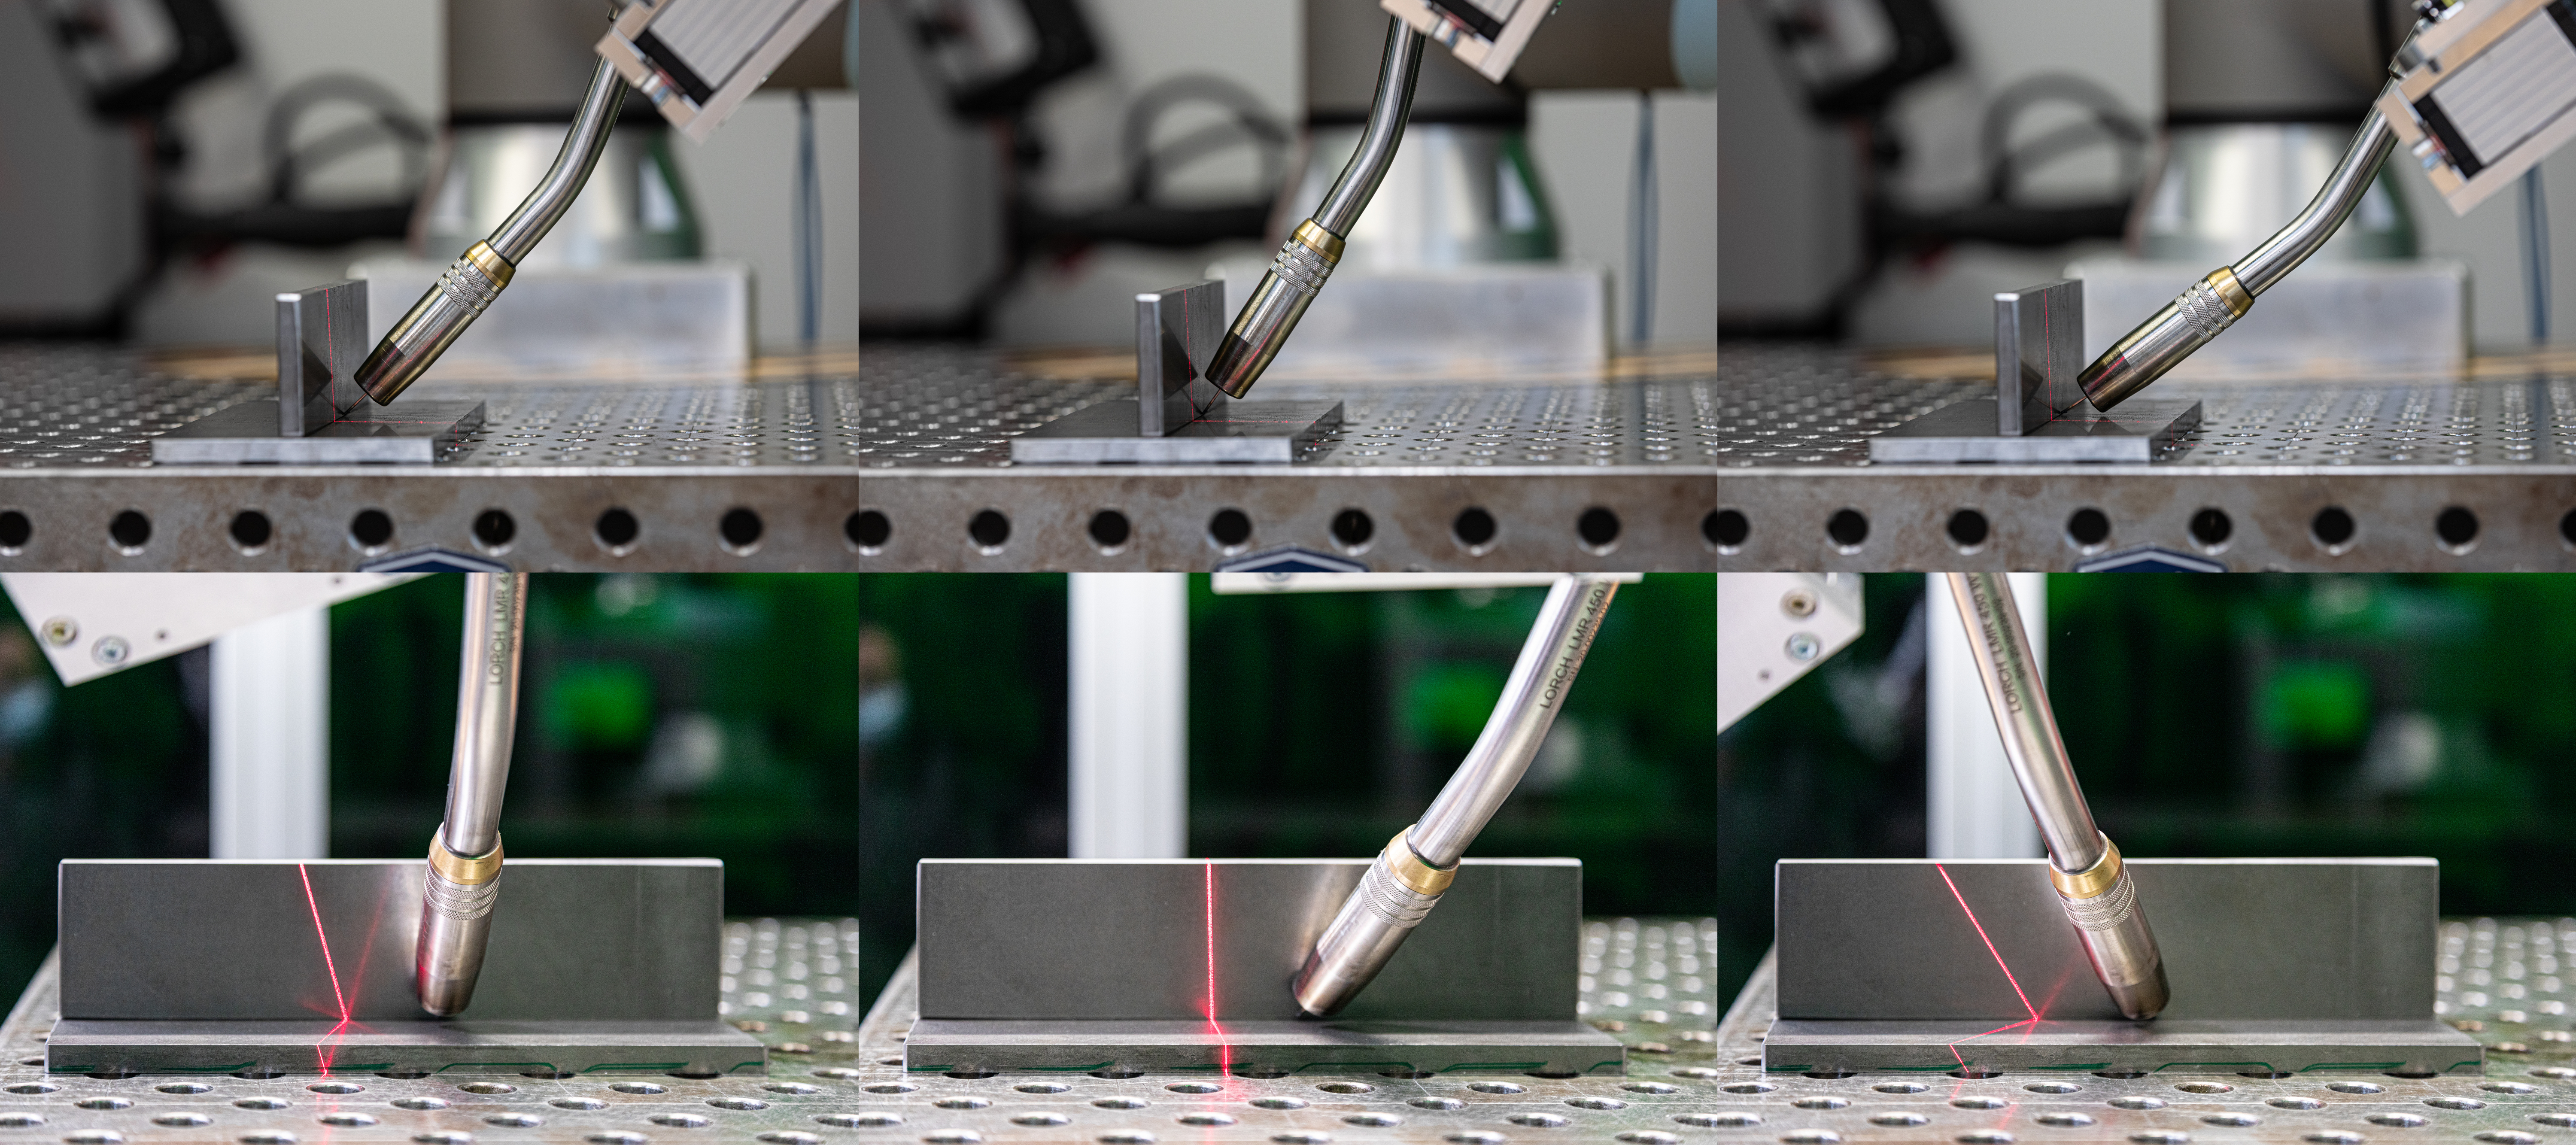
\includegraphics[width=\textwidth]{Abbildungen/collage.jpg}
	\centering
	\caption{Der Laserliniensensor auf einem Werkstück projiziert}
\end{figure}

\section{Software}
Die Erstellung des Softwarepakets namens \emph{processit} zur Realisierung der erzielten Funktion des Schweißroboters ist die Kernarbeit der Fraunhofer IPA. Hierfür wird das ROS-Industrial-Paket aus Abschnitt~\ref{ssec:ros_industrial} als Fundament verwendet. Dies ermöglicht eine einwandfreie Integration des Cobots und enthüllt ein Rahmenwerk für die Kommunikation und Steuerung des Roboters über Programmierschnittstellen. Die komplexe Aufgabe der automatischen Naht-Erkennung und des Schweißens kann in überschaubarer Teilaufgaben zerlegt werden. Bezugnehmend auf Abschnitt~\ref{sec:ROS} können somit Teilaufgaben separat erarbeitet werden und die Aufgabe der Zusammenführung und Koordinierung an ROS überlassen werden.

\subsection{Abstraktion des Softwarepakets}
Bevor die genauen Funktionen der einzelnen Teilmodule angeschaut werden, lohnt sich eine Vereinfachung der komplexen Funktionsweise des ganzen Softwarepakets. Die höhere Softwarearchitektur leitet sich aus der drei vernetzten Geräte und somit drei Kernmodule. Die Software verkoppelt den Roboter, Laserlinienscanner und über das Teach-In-Pendant die Benutzeroberfläche mit einander und verwendet dafür die Pakete \emph{processit\textunderscore sensors}, \emph{processit\textunderscore detection} und \emph{processit\textunderscore adapt}. Das Modul processit\textunderscore sensors ist für Steuerung des Sensors sowie die Vorverarbeitung der Sensordaten zuständig. In die Vorverarbeitung wird das Störgeräusch ausgefiltert und die Koordinaten der Punktewolke zur Weltkoordinaten transformiert. Dieses Koordinatensystem auf das globale System und ist der Bezugspunkt für andere Koordinatensysteme. Diese Information wird an dem nächsten Modul - processit\textunderscore detection - übertragen, welches die Aufgabe der Naht-Erkennung übernimmt. Deren Funktionsweise wird bei der genaueren Behandlung des dafür zuständigen Teilmoduls erklärt. Nach der Erkennung der Naht wird diese Erkenntnis durch \emph{processit\textunderscore adapt} verwendet, um zusammen mit externe Module wie MoveIt eine Bahn für den Roboter auszurechnen. Die geplante Trajektorie wird dem Roboter über einen ROS-Treiber bereitgestellt, der durch den Hersteller zur Verfügung gestellt wird. Dieses Kernmodul kommuniziert auch mit dem Teach-In-Pendant, sodass das Starten der Schweißaufgabe sowie die Parametersetzung des Roboters und Schweißprozesses über die Benutzeroberfläche erfolgen kann. Einen Blick auf den Datenfluss stellt klar, wie der autonome Schweißprozess von der Erkennung bis zur Bahnplanung abgewickelt wird.

\begin{figure}[htp]
	\includegraphics[width = \textwidth]{Abbildungen/data_flow_diagram.png}
	\centering
	\caption{Datenfluss innerhalb processit}
	\label{fig:Datenfluss}
\end{figure}

Die Legende zur Interpretierung von Abbildung~\ref{fig:high-level-architecture} ist im Anhang~\ref{a:legende} zu finden. Ein Verständnis der höheren Funktionsweise von processit dient dem Überblick bei einer Untersuchung der einzelnen Teilmodule, die zur Kernfunktionalitäten des Programmpakets beitragen. 

\begin{figure}[tp]
	\includegraphics[width = \textwidth]{Abbildungen/architecture_rough.png}
	\centering
	\caption{Höhere Softwarearchitektur des processit-Softwarepakets}
	\label{fig:high-level-architecture}
\end{figure}

\subsection{ROS-Module}
Vor einer Betrachtung der einzelnen Teilmodule ist es wichtig, ein paar Konzepte zu diskutieren, die ein wesentliches Aspekt des Entwicklungsprozesses gewesen sind. Die Objektorientierung in der Softwareentwickelung dient zur Verbesserung der Erweiterbarkeit, Testbarkeit und des Wartungsaufwands einer Software. Objektorientierte Ansätze machen Objekte zur Lösung komplexere Probleme zu Nutze. Ein Objekt besteht aus verschiedene Eigenschaften und Funktionen, die Methoden genannt werden, die Alleinstellungsmerkmale des Objekts sind. Diese Eigenschaften und Methoden werden somit mit dem Objekt verbunden und dürfen nur durch ihm verwendet werden. Objekte ermöglichen die Abstrahierung und Modellierung komplexer, vielseitiger Daten und vereinfachen ihrer Anwendung in einer Software. Objekte können in objektorientierten Programmiersprachen mit Klassen erstellt werden. \autocite[27-28]{Lahres2021} \autocite[415-416]{Kaiser2022}

Konzepte wie die lose Kopplung und Abhängigkeitsinjektion sowie -Inversion wurden in der Entwicklung von processit sehr häufig benutzt. Die lose Kopplung ist ein Konzept der serviceorientierten Architektur bei der Softwareentwickelung, die eine Reduzierung des Abhängigkeitsgrad zwei Module oder Objekte beziehungsweise Klassen fördert. Somit können Klassen und Objekte mehr angepasst werden, ohne große Änderungen in den abhängigen Klassen vorzunehmen. Mit einer losen Kopplung ist es möglich, einzelne Objekte nach ihrer Hauptfunktionen zu abstrahieren. Somit ist eine Anwendung unterschiedlicher Objekte mit den gleichen Hauptfunktionen in einer Klasse oder Modul ohne deren beziehungsweise dessen Anpassung möglich. \autocite{Hockkoon2010}

Die Abhängigkeitsinversion ist ein Entwurfsprinzip, wo die Abhängigkeitsrelationen zweier oder mehrerer Module oder Klassen wiederkehrt werden. Somit hängen sie nicht von konkreten Objekte ab, sondern von Abstraktionen  \autocite[67]{Noback2018}. Abhängigkeitsinjektion ist ein Konzept dieses Entwurfsprinzips, welches die Verbesserung der Wiederverwendbarkeit, Wartbarkeit, und Testbarkeit von Software erzielt. Diese Vorgehensweise ermöglicht die Entwicklung von lose-gekoppelter Software, indem Klassen Objekte mit bestimmten Funktionalitäten auffordern können und diese ihnen geliefert werden. Somit reduzieren sich die Verantwortungen der Klasse, indem sie nicht für die Erstellung des erforderten Objektes zuständig ist. \autocite[204-1112]{Gregoire2021}

Zwecks der Wiederverwendbarkeit sind die einzelne Teilmodule von processit als ROS-Module gestaltet. Jedes Modul erstellt nach dem Start je nach Aufgabenvielfalt eigene ROS-Nodes. Innerhalb jedes Moduls werden die Codedateien, die von ROS abhängig sind, von anderen ROS-unabhängigen Codedateien zwecks des Organisierens getrennt.

\subsubsection{processit\textunderscore sensors}
Dieses Modul ist für den Informationsaustausch mit dem Laserliniensensor zuständig. Das Starten und Stoppen sowie die Parametersetzung des Lasers erfolgt über dieses Modul. Ein gesondertes Modul \emph{scanconctrol\textunderscore handler} übernimmt die Funktion als Schnittstelle zwischen dem \emph{processit\textunderscore sensors} Node und ROS Treiber des Sensors. Über ein Control-Register können die Stärke des Lasers und verschiedene Sensorparameter eingestellt werden.

Ein externer ROS-Modul, der einen Treiber für den Laserliniensensor anbietet, wird zur Gewinnung der Geometriedaten in Form einer Punktewolke verwendet. Dieses Modul stellt einen ROS-Publisher bereit, der regelmäßig neue Punktwolken aussendet, während der Laserscanner über das Werkstückprofil verläuft. Dieser Punktewolken sind allerdings Rohdaten und müssen zuerst vorverarbeitet werden und zum Weltkoordinatensystem transformiert werden. Ein Präprozessor ist für diese Aufgabe zuständig. Ein eingebauter ROS-Subscriber abonnierten Punktewolken von dem Treiber, prüft sie auf Datengültigkeit und filtert sie auf Basis einer statistischen Methode. Hierbei werden Punkte entfernt, die innerhalb eines bestimmten Radius nicht eine Mindestanzahl an benachbarten Punkten haben. Nach der Entfernung von Ausreißern wird die Punktewolke in das Weltkoordinatensystem transformiert und mittels eines eingebauten ROS-Publishers für die Weiternutzung zu einem ROS-Topic (\emph{scan\textunderscore world}) veröffentlicht.  

Die Lasersensordaten werden auch in einer Simulation des Roboters in Gazebo simuliert werden, um eine Testumgebung ohne die Einbindung der Hardwarekomponenten zu ermöglichen.

\subsubsection{processit\textunderscore detection} \label{sssec:processit_detection}
Dieses Softwarepaket stellt den vierten Baustein des Datenflusses in Abbildung~\ref{fig:Datenfluss} dar. Hier werden die gefilterten Geometriedaten der Punktewolke verwendet, um eine Naht zu erkennen. Der ROS-Node \emph{scan\textunderscore processor} dient als eine Schnittstelle zur Verbindung mit anderen ROS-Nodes außerhalb dieses ROS-Moduls. Neben seine Rolle als Schnittstelle und Kommunikationsagent steuert er auch den Prozess zur Detektierung der Naht. Die Möglichkeit des Startens, Pausierens, Fortsetzens und Stoppens der Detektion wird auch durch dieser Node in Form von ROS-Services angeboten. Auch die Detektionsmodi, die die Geschwindigkeit und Genauigkeit des Detektionsverfahrens regeln, können über den \emph{scan\textunderscore processor} Node geregelt werden. Die eigentliche Detektion der Naht wird allerdings durch den Prozessor an das jeweilige Erkennungsmodul für den entsprechenden Anwendungsfall delegiert. 

Da es unterschiedliche Arten einer Schweißnaht geben, werden unterschiedliche Verfahren zur Erkennung der Schweißnaht verwendet. Hierbei wird das Entwurfsprinzip der losen Kopplung angewendet. Die Klasse des Detektors wird abstrahiert, sodass mehrere Erkennungsverfahren unter dieser abstrakten Klasse zugeordnet werden können. Somit verfügt der Prozessor beim Abruf der abstrakten Klasse automatisch über die implementierten Erkennungsmethoden und muss nicht situationsabhängig die einzeln aufrufen. Abhängig von der abstrakten Basisklasse wurden Klassen für die Erkennungsverfahren einer Kehlnaht, Stumpfnaht und einer offline erzeugten Werkzeugbahn. Die Erkennung einer vordefinierten Werkzeugbahn ist für das Abfahren einer Freiformfläche notwendig. Die Stumpfnaht-Erkennung und Werkzeugbahn-Erkennung befinden sich gerade in einer Prototyp-Phase. Eine Abstrahierung des Codes zum Verständnis der Struktur ist im Anhang~\ref{a:abstraktion_nahterkennung} zu finden. Der Auswahl einer Erkennungsmethode erfolgt nicht bei der Initialisierung der Klasse, da es bei einer Änderung des Schweißnahttypes ein Neustart des Programms nötig wäre. Stattdessen erfolgt der Auswahl dynamisch über eine Funktion, die die Konfigurationsdaten einliest und eine Wahl trifft. Diese Daten werden als Teil der Request-Nachricht beim aufrufen des Services zum Starten des Detektionsverfahrens erhalten.
´
Schließlich wird zur Aufnahme, Protokollierung und Speicherung der Punktewolke-Daten eine Logger-Klasse implementiert. Diese abonniert ein ROS-Topic namens scan\textunderscore world und erhält somit gleichzeitig wie der \emph{scan\textunderscore processor} die vorverarbeitete Geometrieinformation. Eingebaut ist auch ein ROS-Subscriber, der dem ROS-Topic \emph{stopRecording} abonniert. Diese signalisiert dem Logger über das Ende des Detektionsverfahrens und löst den Speichervorgang der aufgenommenen Punktewolke aus. 

\subsubsection{processit\textunderscore adapt}
Dieses ROS-Modul enthält die wichtigsten Komponenten des processit-Projekts. Es ist die Hauptschnittstelle zur Kommunikation mit der Benutzeroberfläche des Teach-In-Pendants. Ein selbsterstelltes Plugin für die Software des Pendants ermöglicht die Aktivierung der smarten Funktionen von processit. Dieses Plugin kann ROS-Services aufrufen, die sich in diesem Modul befinden und die Roboterbewegung sowie den Schweißprozess steuern. Darüber hinaus können auch Vorgänge zur Kalibrierung und Kommissionierung des Roboters hieraus gestartet werden.

Das \emph{robot\textunderscore controller\textunderscore bridge} funktioniert analog zu einer Brücke zwischen dem ganzen processit-Programmpaket und der Steuereinheit des Roboters. Hierüber kann der Schweißvorgang gesteuert werden, indem gezielt ROS-Services aufgerufen werden. Diese Services sind für vier Hauptaufgaben ausgelegt worden. Ein Service zur Initialisierung des Vorganges wird zuerst aufgerufen. Hier werden unter anderem die, durch den Benutzer gesetzten Parameter eingelesen. Der nächste Service startet eine Vorfahrt des Roboters, die zur Erkennung der Schweißnaht und ihrer Position dient. Danach fängt der eigentliche Schweißprozess an, wo der Roboter die Naht verfolgt. Nach Ende der Naht wird der letzte Service aufgerufen, der den Schweißvorgang beendet. Daneben wird die Kalibrierung des Lasersensors auch in diesem Programm als einen ROS-Service angeboten. Die eigentliche Aufgabe der Aufgabenausführung, Bahnplanung und Kalibrierung wird an anderen Unterprozesse delegiert. 

Ähnlich wie das Detektionsverfahren aus~\ref{sssec:processit_detection}, gibt es unterschiedliche Verfahrensarten zum Schweißen eines Bauteils. Es wird nicht über die Schweißverfahren geredet, sondern die unterschiedlichen Varianten, in der ein Roboter an einer Schweißaufgabe herangehen könnte. Das processit-Paket bietet drei Varianten der Herangehensweisen zum Schweißen eines Bauteils an. Diese werden \emph{task\textunderscore appliers} genannt. Mit dem gleichen Zweck der Simplifizierung wird auch hier das Entwurfsprinzip der losen Kopplung mittels Abhängigkeitsinjektion angewendet. Die Services aus robot\textunderscore controller\textunderscore bridge rufen eine abstrakte Klasse auf, die konkret für die drei Herangehensweisen implementiert wird. Die erste Variante (online\textunderscore following) ist die Online-Verfolgung. Hierbei erfolgt die Erkennung der Naht während einer Bewegung des Roboters. Die Trajektorie des Roboters wird soeben während des Schweißvorganges ermittelt. Es sind hier zwei Bewegungsplaner nötig. Der erste, ein industrieller Bewegungsplaner von Pilz, dient zur Errechnung einer vorläufige Bahn nach der Erkennung der Schweißnaht-Position und Orientierung. Der zweite, ein selbsterstellter Planer, dient der weiteren Planung einer Trajektorie mit Tiefeninformation aus dem Laserliniensensor in echter Zeit. Bei der zweiten Variante (Scan \& Plan) wird zuerst ein Messvorgang durchgeführt. Aus den Erkenntnissen dieses Vorganges wird mit einem Bewegungsplaner eine Trajektorie generiert. Die dritte Variante (toolpath\textunderscore following) ist für das Schweißen einer Freiformoberfläche und ist wie bei dessen Detektionsverfahren in einer Prototyp-Phase. Es gibt eine vierte Variante des Prozesses, die der Kalibrierung des Laserliniensensors dient und für den eigentlichen Schweißprozess wenig relevant ist. Es werden über die Basisklasse auch die ROS-Services für die Detektionsaufgabe aus~\ref{sssec:processit_detection} gestartet und stehen somit erst mit dem Start des Schweißvorganges zur Verfügung. Der Auswahl einer Herangehensweise erfolgt auch hier dynamisch auf Basis der Konfigurationsdaten, die in der Request-Nachricht des aufgerufenen Services stehen. Ein Beispiel zur Veranschaulichung der Code-Struktur ist im Anhang unter %TODO: add ref to appendix

Innerhalb der einzelnen Implementationen wird die Aufgabe der Bahngenerierung für den Roboter weiter delegiert. Bei der Erstellung einer Bahn wird die Pose der Schweißnaht rechnerisch ermittelt. Es wird die Tiefeninformation der Schweißnaht benutzt, die der Detektionsprozess aus~\ref{sssec:processit_detection} gewonnen wird, um die Position und Orientierung der Schweißnaht zu erkennen. Für jede Herangehensweise sind Generatoren zuständig, die mit Hinsicht auf die speziellen Anforderungen jeder Variante erstellt wurden. Diese werden \emph{path\textunderscore generators} genannt. Unter Verwendung des gleichen Prinzips der Abhängigkeitsinversion wird auch hier eine abstrakte Klasse erstellt, die in den einzelnen Implementationen konkretisiert wird. Wie bei den task\textunderscore appliers wird die Bahngenerierung auch für das online\textunderscore following, das Scan \& Plan, toolpath\textunderscore following und den Kalibriervorgang des Laserliniensensors implementiert. Eine Veranschaulichung der Code-Struktur ist im Anhang unter %TODO: add ref to appendix

Ein detaillierter Programmablauf der obigen Module ist im Anhang~\ref{a:processit_detailablauf} zu finden. Diese drei Hauptmodule des processit-Pakets werden durch weitere Stützmodule ergänzt, die verschiedene Aufgaben der Simulation, Bahnplanung, Visualisierung und jeglicher Berechnungen übernehmen. Die effektive Zusammenarbeit der drei Hauptmodule sowie Stützmodule funktioniert nur mit der effektiven Kommunikation zwischen diesen Modulen. Deswegen werden zunächst die unterschiedlichen ROS-Messages diskutiert, die den Kernpartikel der zwischen-modularen Kommunikation bilden.


\subsection{ROS-Messages von processit}
Die in processit verwendeten ROS-Messages können grundsätzlich nach ihrer Verwendung unterschieden werden. Es werden für die Publisher-Subscriber-Kommunikation innerhalb von ROS Nachrichten verwendet sowie als Austauschmittel zwischen Clients und Servers. Die Behandlung aller ROS-Messages beider Arten wird zu umfangreich und ist nicht das Ziel dieses Abschnitts. Es werden nur die kritischen Nachrichtenarten behandelt, die zum Verständnis der Kommunikation zwischen den Hauptprozessen sind. 

Es werden zuerst die ROS-Messages angeschaut, die Information aus Sensoren des Robotersystems vermitteln. Die ROS-Message \emph{PointCloud2} enthält Information über die Punktewolke, die aus der Messwerte des Laserliniensensors erstellt wird. Dies enthält nicht nur die Punktwolke selbst, sondern auch Metadaten dazu. Darunter zählt die Aufnahmezeit der Punktewolke, deren Höhe sowie Breite, und die Datengültigkeit der Punktewolke unter anderem. Die Lage der Robotergelenke aus den internen Sensoren steht auch den ROS-Modulen in Form einer ROS-Message zur Verfügung. \emph{JointState} speichert Daten über die Position, Geschwindigkeit, und Belastungsgrad eines Gelenks, das über einen einzigartigen Namen identifiziert wird. Die Rohdaten aus einem Laserscan werden in einer ROS-Message namens \emph{LaserScan} gespeichert, die nicht nur die Messwerte in Form von Abständen enthält, sondern auch Metadaten wie der Winkel am Anfang und Ende des Scans, die Dauer und die Grenzwerte der Messungen. Aus der Information dieser ROS-Message kann eine Punktewolke auf Basis der PointCloud2 ROS-Message erstellt werden.

Als nächstes werden ROS-Messages betrachtet, die geometrische Information enthalten. Ein paar grundlegende Messages müssen zuerst definiert werden, da sie häufig in anderen ROS-Messages eingebettet werden. Die ROS-Message \emph{Vector3} wird zur Sendung von dreidimensionaler Vektorinformation verwendet. Vector3 wird für den Ausdruck einer räumlichen Geschwindigkeit als linearer- und Winkelgeschwindigkeit in der \emph{TwistStamped} Message angewendet. Die Koordinatentransformationen zwischen den einzelnen Komponenten des Robotersystems sowie den Gelenken des Roboters werden auch über ROS-Messages ausgetauscht. Eine Koordinatentransformation wird in einer ROS-Message namens \emph{transform} gespeichert, die Details über die translatorische und rotatorische Transformation als Vektoren und Quaternionen enthält. Diese Message wird kaum eigenständig verwendet, sondern in einer \emph{TransformStamped} Message eingebettet. Diese Message enthält zusätzliche Header-Daten, die eine ID des Eltern-Koordinatensystems hat, und die Identifikation des Koordinatensystems, das sich auf dem Eltern-Koordinatensystem bezieht. Auch geometrische Information über eine Pose wird als eine ROS-Message strukturiert. Diese enthält Details über eine Position als einen Punkt in einem dreidimensionalen Raum und die Orientierung des Punktes als eine Quaternion. 

ROS-Messages können auch zur Bekanntgabe von Details über den Roboter verwendet werden. In der Message \emph{RobotState} werden Details über die Position von Gelenke und Armteile sowie Objekte mit Kollisionsgefahr kompiliert. In der \emph{RobotTrajectory} ROS-Message sind Auskünfte über die aktuelle Bahn der Robotergelenke enthalten. Weitere ROS-Messages bestehen auch zur Übermittlung von Information über Trajektorien. Diese Information stellt sich aus dem Bahnverlauf, der Geschwindigkeit, Beschleunigung und dem Ruck zusammen. 

Viele Aktionen des processit-Pakets werden durch ROS-Services ausgelöst. ROS-Services erhalten Anfragen und senden Antworten in Form von Nachrichten. Hierfür werden auch ROS-Messages verwendet. Die Parametersetzung des Laserliniensensors erfolgt über einen ROS-Service. Hierzu wird eine Anfrage gesendet, die Angaben zu der Laserfrequenz, Belichtungszeit und Operationsmodus enthält. Bei dem Aufruf dieses Services wird keine Antwort gesendet. Auch zum Starten des Detektionsverfahrens aus Abschnitt~\ref{sssec:processit_detection} wird eine Abfrage gesendet. Diese enthält Auskünfte über die zu suchende Geometrie (eine Kehlnaht oder Stumpfnaht), eine Identifikationszeichenkette, die kartesische Trajektorie, die Pose des Startpunkts und eine Reihe weiterer Posen, die für das Schweißen einer Freiformoberfläche wichtig sind. Als eine Antwort nach der Ausführung wird eine Statusnachricht über den Prozesserfolg erhalten. Der Service zur Initialisierung des Schweißvorganges erhält eine detailreiche Anfrage. In dieser Nachricht ist Information über die zu schweißende Geometrie, Bewegungssteuerende Eigenschaften wie die Geschwindigkeit und andere prozessrelevante Details enthalten. Als Antwort wird hier auch eine Statusnachricht über den Prozesserfolg erhalten. Zum Fortsetzen des Schweißvorganges nach einer Pause wird auch eine Anfrage zu dem zuständigen ROS-Service gesendet. Da alle prozessrelevante Details in der Anfrage für die Prozessinitialisierung gesendet wurden, steht in dieser Anfrage nichts. Auch dieser Service sendet eine Statusnachricht über den Prozesserfolg zurück. Der \emph{AddPoseMarker} ROS-Service ist speziell für die Werkzeugbahnverfolgung bei dem Schweißen einer Freiformoberfläche ausgelegt. Er wird zur Setzung von virtueller Markierungen auf der Werkzeugbahn verwendet. Dieser erhält per Anfrage verschiedene geometrische sowie andere prozessrelevante Details und sendet eine einzigartige Identifikation für die gesetzte Markierung. 

Viele dieser ROS-Messages werden durch externe Module sowie Stützmodule des processit-Pakets verwendet, um Funktionen innerhalb des Programmpakets aufzurufen oder mit dem Programm zu kommunizieren.

%\subsection{Support-Module} \label{ssec: support_modules}
%Die Stützmodule des Programmpakets bieten zusätzliche Funktionalitäten an. Es können die Sensormessungen und Roboterbewegungen visualisiert werden. Die Berechnung einer Trajektorie für den Roboter wird auch durch ein Stützmodul übernommen. Letztlich kann das Verhalten des Robotersystems mittels einer Simulationsumgebung auch detailliert getestet werden, welches besonders hilfreich bei dem Testen neuer Funktionalitäten ist. Hierfür werden die diversen Zusatzmodule von ROS aus Abschnitt~\ref{sec:ROS} verwendet.
%
%Mittels Rviz kann nicht nur die Roboterbewegung in seiner Umgebung überwacht werden, sondern auch die Messungen des Lasersensors. Diese werden innerhalb von processit\textunderscore sensors bearbeitet, sodass sie durch das Rviz Programm visualisiert werden können. Mittels STL-Dateien wird die Geometrie der Einzelkomponenten des Robotersystems dem Rviz-Programm übermittelt. Hierunter zählt nicht nur der Roboter und seiner Umgebung, sondern auch der Laserliniensensor und die Schweißpistole. Diese werden möglichst präzise modelliert. Die Visualisierung der Einzelkomponenten sowie der Sensor- und Koordinateninformation kann mittels Konfigurationsdateien in Rviz angepasst werden. Die Integration von Rviz in dem processit-Programmpaket ermöglicht die Prozessüberwachung aus der Roboter-Sichtweise und dient dem Verstehen des Roboterverhaltens während eines Programmablaufs. 
%
%Das Programm Gazebo wird als eine Simulationsumgebung für das processit-Programmpaket verwendet. Dieses Programm wird für die Erschaffung eines digitalen Zwilling für das Robotersystem verwendet. Es können virtuelle Bauteile in der Simulationsumgebung eingeladen werden, die virtuell durch den Roboter verarbeitet werden können. In dieser Umgebung werden auch die physikalischen Zusammenhänge der physischen Komponenten vordefiniert, sodass die Bewegung des Roboters möglichst realitätsnah abgebildet werden kann. Auch Sensoren wie der Laserliniensensor werden hier modelliert und sind dazu fähig, das virtuelle Bauteil optisch anzutasten und Sensorwerte in Form der ROS-Message, LaserScan, zu emulieren. Ähnlich wie Rviz erfolgt die Einstellung von Gazebo mittels 3D-Objektdateien wie STL-Dateien und Konfigurationsdateien in form von YAML- sowie XML-Dateien. 
%
%Andere Module wie das \emph{ur\textunderscore robot\textunderscore driver} und MoveIt dienen unterschiedliche Zwecke zur Realisierung der Roboterfunktion. das ur\textunderscore robot\textunderscore driver agiert als einen ROS-Treiber für die Robotersteuerung und ermöglicht die Kommunikation zwischen den beiden Teilen. MoveIt wird zur Planung verschiedener Trajektorien des Roboters verwendet. Diese Module ersparen viel Aufwand und Zeit für den Entwicklern des processit-Programmpakets und lassen sie auf das wesentliche konzentrieren. 
